\documentclass[10pt,a4paper]{article}
\usepackage[utf8]{inputenc}
\usepackage[english]{babel}
\usepackage[activate={true,nocompatibility},final,tracking=true,kerning=true,spacing=true]{microtype}
\usepackage{fullpage}
\usepackage{graphicx}
\usepackage{fancyhdr}
\usepackage{occi}
\setlength{\headheight}{13pt}
\pagestyle{fancy}

%  just a test
% default sans-serif
\renewcommand{\familydefault}{\sfdefault}

% no lines for headers and footers
\renewcommand{\headrulewidth}{0pt}
\renewcommand{\footrulewidth}{0pt}

% header
\fancyhf{}
\lhead{GFD-P-R.184}
\rhead{\today}

% footer
\lfoot{occi-wg@ogf.org}
\rfoot{\thepage}

% paragraphs need some space...
\setlength{\parindent}{0pt}
\setlength{\parskip}{1ex plus 0.5ex minus 0.2ex}

%\renewcommand\paragraph{%
%  \@startsection{paragraph}{4}{0mm}%
%     {-\baselineskip}%
%     {.5\baselineskip}%
%     {\normalfont\normalsize\bfseries}}

% some space between header and text...
\headsep 13pt

\setcounter{secnumdepth}{4}

\begin{document}

% header on first page is different
\thispagestyle{empty}

Draft \hfill  Thijs Metsch, Intel\\
OCCI-WG \hfill  Andy Edmonds, ICCLab, ZHAW\\
\rightline {October 7, 2010}\\
\rightline {Updated: \today}

\vspace*{0.5in}

\begin{Large}
\textbf{Open Cloud Computing Interface - Infrastructure}
\end{Large}

\vspace*{0.5in}

\underline{Status of this Document}

% This document provides information to the community regarding the
specification of the Open Cloud Computing Interface. Distribution is
unlimited.


This document is a \underline{draft} including proposed errata updates
to the OCCI Infrastructure \cite{occi:infrastructure} specification.

The errata updates are summarized in section~\ref{sec:errata}.

Eventually this document will obsolete GFD-P-R.143. This document is
fully backward compatible to \cite{occi:infrastructure}.

\underline{Copyright Notice}

Copyright \copyright ~Open Grid Forum (2009-2015). All Rights
Reserved.

\underline{Trademarks}

OCCI is a trademark of the Open Grid Forum.

\underline{Abstract}

This document, part of a document series, produced by the OCCI working
group within the Open Grid Forum (OGF), provides a high-level
definition of a Protocol and API. The document is based upon
previously gathered requirements and focuses on the scope of important
capabilities required to support modern service offerings.


\newpage
\tableofcontents
\newpage

\section{Introduction}
The Open Cloud Computing Interface (OCCI) is a RESTful Protocol and
API for all kinds of management tasks. OCCI was originally initiated
to create a remote management API for IaaS%
\footnote{Infrastructure as a Service}
model-based services, allowing for the development of interoperable tools for
common tasks including deployment, autonomic scaling and monitoring.
%
It has since evolved into an flexible API with a strong focus on
interoperability while still offering a high degree of extensibility. The
current release of the Open Cloud Computing Interface is suitable to serve many
other models in addition to IaaS, including e.g.~PaaS and SaaS.

In order to be modular and extensible the current OCCI specification is
released as a suite of complimentary documents, which together form the complete
specification.
%
The documents are divided into three categories consisting of the OCCI Core,
the OCCI Renderings and the OCCI Extensions.
%
\begin{itemize}
\item The OCCI Core specification consists of a single document defining the
 OCCI Core Model. The OCCI Core Model can be interacted with {\em
 renderings} (including associated behaviours) and expanded through {\em extensions}.
\item The OCCI Rendering specifications consist of multiple documents each
 describing a particular rendering of the OCCI Core Model. Multiple renderings can
 interact with the same instance of the OCCI Core Model and will automatically support
 any additions to the model which follow the extension rules defined in OCCI
 Core.
\item The OCCI Extension specifications consist of multiple documents each
 describing a particular extension of the OCCI Core Model. The extension documents
 describe additions to the OCCI Core Model defined within the OCCI specification
 suite.
\end{itemize}
%
The current specification consist of three documents.
Future releases of OCCI may include additional rendering and extension
specifications. The documents of the current OCCI specification suite are:

\begin{description}
\item[OCCI Core] describes the formal definition of the the OCCI Core Model
\cite{occi:core}.
\item[OCCI HTTP Rendering] defines how to interact with the OCCI Core Model using the
RESTful OCCI API \cite{occi:http_rendering}. The document defines how the OCCI Core Model can
be communicated and thus serialised using the HTTP protocol.
\item[OCCI Infrastructure] contains the definition of the OCCI Infrastructure
extension for the IaaS domain \cite{occi:infrastructure}. The document defines
additional resource types, their attributes and the actions that can be taken
on each resource type.
\end{description}


OCCI makes an ideal interoperable boundary interface between the web
and the internal resource management system of infrastructure
providers.

\section{Notational Conventions}
All these parts and the information within are mandatory for
implementors (unless otherwise specified). The key words "MUST", "MUST
NOT", "REQUIRED", "SHALL", "SHALL NOT", "SHOULD", "SHOULD NOT",
"RECOMMENDED", "MAY", and "OPTIONAL" in this document are to be
interpreted as described in RFC 2119 \cite{rfc2119}.

\textbf{Andy: we need to state that this document as part of the current document set,
supersedes all previous documents.}


% begin infrastructure content

\section{Infrastructure}
The OCCI Infrastructure document details how an OCCI implementation
can model and implement an Infrastructure as a Service API offering by
utilising the OCCI Core Model. This API allows for the creation and
management of typical resources associated with an IaaS service, for
example, creating a \hl{Compute} instance and \hl{Storage} instance
and then linking them with \hl{StorageLink}. The main infrastructure
types defined within OCCI Infrastructure are:

\begin{description}
\item[\hl{Compute}] Information processing resources.
\item[\hl{Network}] Interconnection resource and represents a L2
  networking resource. This is complimented by the \hl{IPNetwork}
  \hl{Mixin}.
\item[\hl{Storage}] Information recording resources.
\end{description}

Supporting these Resource types are the following \hl{Link} sub-types:

\begin{description}
\item[\hl{NetworkInterface}] connects a \hl{Compute} instance to a
  \hl{Network} instance. This complimented by an
  \hl{IPNetworkInterface} \hl{Mixin}.
\item[\hl{StorageLink}] connects a \hl{Compute} instance to a
  \hl{Storage} instance.
\end{description}

\begin{figure}[!h]
	{\centering \resizebox*{0.9\columnwidth}{!}{\rotatebox{0}
	{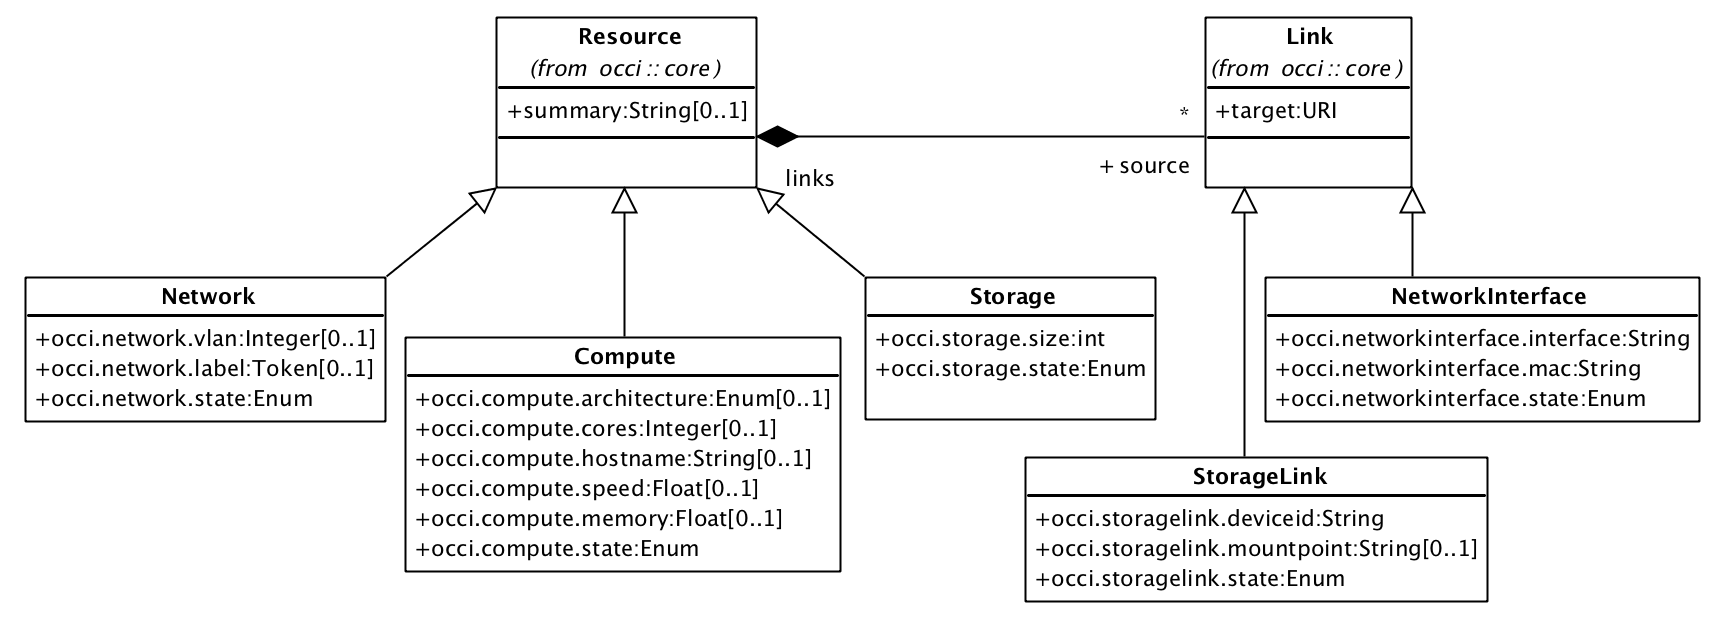
\includegraphics[scale=0.4]{figs/infrastructure_model.png}}} \par}
	\caption{Overview Diagram of OCCI Infrastructure Types.}
	\label{fig:infra_uml}
\end{figure}

These infrastructure types inherit the OCCI Core Model \hl{Resource}
base type and all their attributes. The HTTP Rendering document
\cite{occi:http_rendering} defines how to serialise and interact with
these types using RESTful communication. Implementers are free to
choose what \hl{Resource} and \hl{Link} sub-types to implement. Those
that are supported by an implementation will be discoverable through
the OCCI Query Interface.

As REQUIRED by the OCCI Core Model specification, every type
instantiated that is a sub-type of \hl{Resource} or \hl{Link} MUST be
assigned a \hl{Kind} that identifies the instantiated type. Each such
\hl{Kind} instance MUST be related to the \hl{Resource} or \hl{Link}
base type's \hl{Kind} by setting the \textit{parent} attribute.
 That assigned \hl{Kind} instance MUST always
remain immutable to any client.

\mytablefloat{
	\label{tbl:kinds}The \hl{Kind} instances defined for
	the infrastructure sub-types of \hl{Resource}, \hl{Link} and related \hl{Mixin}s.
	The base URL {\bf http://schemas.ogf.org/occi} has been replaced with
	{\bf $<$schema$>$} in this table for a better readability experience.
	} {
	\begin{tabular}{llll}
	\toprule
	Term & Scheme & Title & Parent \hl{Kind} \\
	\colrule
	compute &  $<$schema$>$/infrastructure\# & Compute \hl{Resource}
	& $<$schema$>$/core\#resource \\

	storage & $<$schema$>$/infrastructure\# & Storage \hl{Resource}
	& $<$schema$>$/core\#resource \\

	storagelink & $<$schema$>$/infrastructure\# & StorageLink \hl{Link}
	& $<$schema$>$/core\#link \\

	network & $<$schema$>$/infrastructure\# & Network \hl{Resource}
	& $<$schema$>$/core\#resource \\

	networkinterface & $<$schema$>$/infrastructure\# & NetworkInterface \hl{Link}
	& $<$schema$>$/core\#link \\

	\botrule
	\end{tabular}
}

Table~\ref{tbl:kinds} describes the \hl{Kind} instances defined for
each of the infrastructure \hl{Resource} or \hl{Link} sub-types. For
information on extending these types, please refer to the OCCI Core
Model document \cite{occi:core}.

The following sections on \hl{Compute}, \hl{Storage} and \hl{Network}
types detail the \hl{Attribute}s, \hl{Actions} and states defined for
each of them, including type-specific mixins where appropriate.
Following those, the definition of infrastructure-related \hl{Link}
sub-types are given and finally OS and Resource Templates
are defined. Figure~\ref{fig:infra_uml} gives an overview of
the key types involved in this infrastructure specification.

\subsection{Compute}
The \hl{Compute} type represents a generic information processing
resource, e.g.~a virtual machine or container. \hl{Compute} inherits
the \hl{Resource} base type defined in OCCI Core Model
\cite{occi:core}.  \hl{Compute} is assigned the \hl{Kind} instance
\textit{http://schemas.ogf.org/occi/infrastructure\#compute}.  A
\hl{Compute} instance MUST use and expose this \hl{Kind}.

\mytablefloat{
	\label{tbl:compute}\hl{Attribute}s defined for the \hl{Compute} type.
}
{
	\begin{tabular}{lp{2.5cm}p{1cm}lp{5cm}}
	\toprule
	Attribute&Type&Multi\-plicity&Mutability&Description\\
	\colrule
	occi.compute.architecture & Enum \{x86, x64\} & 0\ldots1
	& Mutable & CPU Architecture of the instance.\\
	occi.compute.cores & Integer & 0\ldots1
	& Mutable & Number of virtual CPU cores assigned to the instance.\\
	occi.compute.hostname & String & 0\ldots1
	& Mutable & Fully Qualified DNS hostname for the instance.\\
	occi.compute.share & Integer & 0\ldots1
	& Mutable & Relative number of CPU shares for the instance.\\
	occi.compute.memory & Float, ${\mathbf 10}^9$ (GiB) & 0\ldots1
	& Mutable & Maximum RAM in gigabytes allocated to the instance.\\
	occi.compute.state & Enum \{active, inactive, suspended, error\} & 1
	& Immutable & Current state of the instance.\\
	occi.compute.state.message & String & 0..1
	& Immutable & Human-readable explanation of the current instance state.\\
	\botrule
	\end{tabular}
}

Table~\ref{tbl:compute} describes the OCCI Attributes%
\footnote{See the ``{\tt attributes}'' attribute defined by the
  \hl{Category} type and inherited by \hl{Kind} \cite{occi:core}.}
defined by \hl{Compute} through its \hl{Kind} instance. These attributes
MAY or MUST be exposed by an instance of the \hl{Compute} type
depending on the ``Multiplicity'' column in the aforementioned table.

\mytablefloat{
	\label{tbl:compute_actions}%
	\hl{Action}s applicable to instances of the \hl{Compute} type. The
	\hl{Action}s are defined by the \hl{Kind} instance
	\textit{http://schemas.ogf.org/occi/infrastructure\#compute}. Every \hl{Action}
	instance in the table uses the
	\textit{http://schemas.ogf.org/occi/infrastructure/compute/action\#}
	categorisation scheme. ``Action Term'' below refers to \hl{Action}.{\tt term}.
}
{
	\begin{tabular}{lll}
	\toprule
	Action Term & Target state & Attributes \\
	\colrule
	start & active & -- \\
	stop & inactive & method=\{graceful, acpioff, poweroff\} \\
	restart & active (via stop and start chain) & method=\{graceful, warm, cold\} \\
	suspend & suspended & method=\{hibernate, suspend\} \\
	\botrule
	\end{tabular}
}

Table~\ref{tbl:compute_actions} describes the \hl{Action}s defined for
\hl{Compute} by its \hl{Kind} instance. These \hl{Action}s MUST be
exposed by an instance of the \hl{Compute} type of an OCCI
implementation.  Figure~\ref{fig:compute_state} illustrates the state
diagram for a \hl{Compute} instance.

\begin{figure}[!h]
	\centering
	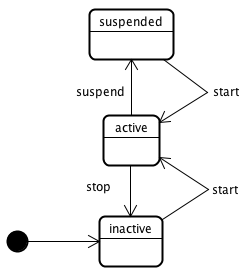
\includegraphics[scale=0.4]{figs/compute-state.png}
	\caption{State Diagram for a \hl{Compute} instance.}
	\label{fig:compute_state}
\end{figure}

\subsection{Network}
The \hl{Network} type represents a L2 networking entity (e.g.~a
virtual switch). It can be extended using the mixin mechanism (or
sub-typed) to support L3/L4 capabilities such as TCP/IP etc.  For the
purposes of this specification we define an OCCI mixin so that IP
networking can be supported where required. \hl{Network} inherits the
\hl{Resource} base type defined in OCCI Core Model \cite{occi:core}.

The \hl{Network} type is assigned the
\textit{http://schemas.ogf.org/occi/infrastructure\#network}
\hl{Kind}. A \hl{Network} instance MUST use and expose this \hl{Kind}.

\mytablefloat{
	\label{tbl:network}\hl{Attribute}s defined for the \hl{Network} type.
}
{
	\begin{tabular}{lp{2.5cm}p{1cm}lp{5cm}}
	\toprule
	Attribute&Type&Multi\-plicity&Mutability&Description\\
	\colrule
	occi.network.vlan & Integer: 0-4095 & 0\ldots1 & Mutable
	& 802.1q VLAN Ientifier (e.g. 343).\\
	occi.network.label & Token & 0\ldots1 & Mutable
	& Tag based VLANs (e.g. external-dmz).\\
	occi.network.state & Enum \{active, inactive, error\} & 1 & Immutable
	& Current state of the instance.\\
	occi.network.state.message & String & 0..1 & Immutable
	& Human-readable explanation of the current instance state.\\
	\botrule
	\end{tabular}
}

Table~\ref{tbl:network} describes the OCCI Attributes%
\footnote{See the ``{\tt attributes}'' attribute defined by the
  \hl{Category} type and inherited by \hl{Kind} \cite{occi:core}.}
defined by \hl{Network} through its \hl{Kind} instance. These attributes
MAY or MUST be exposed by an instance of the \hl{Network} type
depending on the ``Multiplicity'' column in the aforementioned table.

\mytablefloat{
	\label{tbl:network_actions}%
	\hl{Action}s applicable to instances of the \hl{Network} type. The
	\hl{Action}s are defined by the \hl{Kind} instance
	\textit{http://schemas.ogf.org/occi/infrastructure\#network}. Every \hl{Action}
	instance in the table uses the
	\textit{http://schemas.ogf.org/occi/infrastructure/network/action\#}
	categorisation scheme. ``Action Term'' below refers to \hl{Action}.{\tt term}.
}
{
	\begin{tabular}{lll}
	\toprule
	Action Term&Target State&Attributes\\
	\colrule
	up & active & --\\
	down & inactive & --\\
	\botrule
	\end{tabular}
}

Table~\ref{tbl:network_actions} describes the \hl{Action}s defined for
\hl{Network} by its \hl{Kind} instance. These \hl{Action}s MUST be
exposed by an instance of the \hl{Network} type of an OCCI
implementation.  Figure~\ref{fig:network_state} illustrates the state
diagram for a \hl{Network} instance.

\begin{figure}[!h]
	\centering
	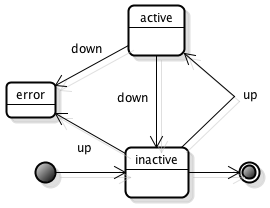
\includegraphics[scale=0.4]{figs/network-state.png}
	\caption{State Diagram for a \hl{Network} instance.}
	\label{fig:network_state}
\end{figure}

\subsubsection{IPNetworking Mixin}

In order to support L3/L4 capabilities (e.g. IP, TCP etc.) an OCCI
mixin is herewith defined.

The \hl{IPNetworking} mixin is assigned%
\footnote{Both assignments use data members from the inherited
  \hl{Category} type \cite{occi:core}.}  the ``{\tt scheme}'' of
\textit{http://schemas.ogf.org/occi/infrastructure/network\#} and the
``{\tt term}'' value \textit{ipnetwork}. An \hl{IPNetworking} mixin
MUST support these values.

Table~\ref{tbl:ipnetworking} define the attributes introduced by the
\hl{IPNetworking} mixin.

The \hl{IPNetworking} mixin MUST be related to the \hl{Network} kind
by setting the \textit{applies} attribute to:

\textit{http://schemas.ogf.org/occi/infrastructure\#network}.

A \hl{Network} instance associated with the
\hl{IPNetworking} mixin \hl{Mixin} instance MUST implement these
attributes.

\mytablefloat{
	\label{tbl:ipnetworking}%
	\hl{Attribute}s defined by the \hl{IPNetworking} mixin. A \hl{Network}
	instance associated with this \hl{Mixin} instance MUST expose these
	attributes.
}{
\begin{tabular}{lp{3.4cm}p{1cm}lp{5.0cm}}
\toprule
Attribute&Type&Multi\-plicity&Mutability&Description\\
\colrule
occi.network.address & IPv4 or IPv6 Address range, CIDR notation & 0\ldots1 & Mutable & Internet Protocol(IP) network address (e.g. 192.168.0.1/24, fc00::/7)\\
occi.network.gateway & IPv4 or IPv6 Address & 0\ldots1 & Mutable & Internet Protocol(IP) network address (e.g. 192.168.0.1, fc00::)\\
occi.network.allocation & Enum \{dynamic, static\} & 0\ldots1 & Mutable & Address allocation mechanism: \textit{dynamic} e.g.~uses the dynamic host configuration protocol, \textit{static} e.g.~uses user supplied static network configurations.\\
\botrule
\end{tabular}
}

In Figure \ref{fig:network_mixin} a UML object diagram depicts how
\hl{Network} would be associated with an IPNetwork \hl{Mixin} when
both are instantiated.

\begin{figure}[!h]
	\centering
	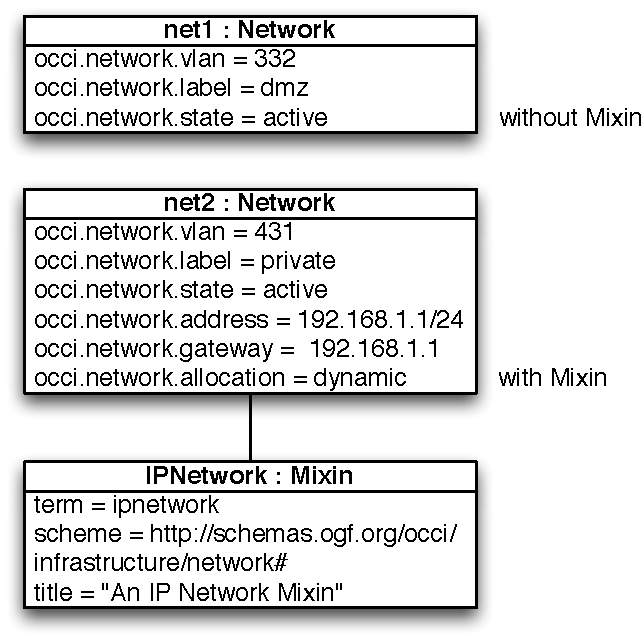
\includegraphics[scale=0.5]{figs/infrastructure_mixins_obj_dia1_network}
	\caption{Object Diagram of a \hl{Network} Instance and its
	Associated \hl{IPNetwork} \hl{Mixin}.}
	\label{fig:network_mixin}
\end{figure}

\subsection{Storage}
The \hl{Storage} type represent resources that record information to a
data storage device.  \hl{Storage} inherits the \hl{Resource} base
type defined in the OCCI Core Model \cite{occi:core}.  The
\hl{Storage} type is assigned the \hl{Kind} instance
\textit{http://schemas.ogf.org/occi/infrastructure\#storage}.  A
\hl{Storage} instance MUST use and expose this \hl{Kind}.

\mytablefloat{
	\label{tbl:storage}\hl{Attribute}s defined for the \hl{Storage} type.
}
{
	\begin{tabular}{lp{2.5cm}p{1cm}lp{5cm}}
	\toprule
	Attribute&Type&Multi\-plicity&Mutability&Description\\
	\colrule
	occi.storage.size & Float, ${\mathbf 10}^9$ (GiB) & 1 & Mutable
	& Storage size in gigabytes of the 	instance.\\
	occi.storage.state & Enum \{online, off\-line, error\} & 1 & Immutable
	& Current status of the instance.\\
	occi.storage.state.message & String & 0..1 & Immutable
	& Human-readable explanation of the current instance state.\\
	\botrule
	\end{tabular}
}

Table~\ref{tbl:storage} describes the OCCI Attributes%
\footnote{See the ``{\tt attributes}'' attribute defined by the
  \hl{Category} type and inherited by \hl{Kind} \cite{occi:core}.}
defined by \hl{Storage} through its \hl{Kind} instance. These attributes
MAY or MUST be exposed by an instance of the \hl{Storage} type
depending on the ``Multiplicity'' column in the aforementioned table.

\mytablefloat{
	\label{tbl:storage_actions}%
	\hl{Action}s applicable to instances of the \hl{Storage} type. The
	\hl{Action}s are defined by the \hl{Kind} instance
	\textit{http://schemas.ogf.org/occi/infrastructure\#storage}. Every \hl{Action}
	instance in the table uses the
	\textit{http://schemas.ogf.org/occi/infrastructure/storage/action\#}
	categorisation scheme. ``Action Term'' below refers to \hl{Action}.{\tt term}.
}
{
	\begin{tabular}{lll}
	\toprule
	Action Term&Target State&Attributes\\
	\colrule
	online & online & --\\
	offline & offline & --\\
%	\botrule
	\end{tabular}
}

Table~\ref{tbl:storage_actions} describes the \hl{Action}s defined for
\hl{Storage} by its \hl{Kind} instance. These \hl{Action}s MUST be
exposed by an instance of the \hl{Storage} type of an OCCI
implementation.  Figure~\ref{fig:storage_state} illustrates the state
diagram for a \hl{Storage} instance.

\begin{figure}[!h]
	\centering
	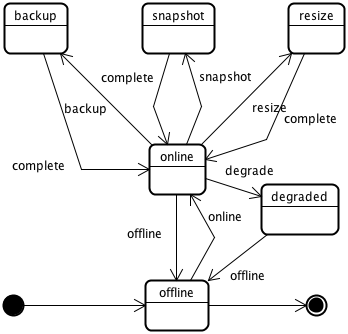
\includegraphics[scale=0.4]{figs/storage-state.png}
	\caption{State Diagram for a \hl{Storage} instance.}
	\label{fig:storage_state}
\end{figure}

OCCI can be used in conjunction with the SNIA cloud storage standard,
Cloud Data Management Interface (CDMI) \cite{cdmi} to provide enhanced
management of the cloud computing storage and data. For storage
managed through CDMI, see the section on \hl{StorageLink}

\subsection{Linking Infrastructure Resources}
In order to create entities like virtual data centres or virtual
clusters, it is necessary to allow the linkage of the previously
defined infrastructure \hl{Resource} sub-types. This is accomplished
by extending (sub-typing) the OCCI Core Model \hl{Link} base type.
This is done as the \hl{Link} base type cannot fully represent
specific types of infrastructure links (e.g.~links to storage or
networks).  These infrastructure links require additional attributes
(e.g.  network interface name) which can only be supported by
sub-typing the \hl{Link} base type.

\subsubsection{Linking to Network}
The \hl{NetworkInterface} type represents an L2 client device (e.g.
network adapter). It can be extended using the mix-in mechanism or
sub-typed to support L3/L4 capabilities such as TCP/IP etc.
\hl{NetworkInterface} inherits the \hl{Link} base type defined in the
OCCI Core Model \cite{occi:core}.

The \hl{NetworkInterface} type is assigned the \hl{Kind} instance
\textit{http://schemas.ogf.org/occi/infrastructure\#networkinterface}.
A \hl{NetworkInterface} instance MUST use and expose this \hl{Kind}.
The \hl{Kind} instance assigned to the \hl{NetworkInterface} type MUST
be related to the \textit{http://schemas.ogf.org/occi/core\#link}
\hl{Kind} by setting the \textit{parent} attribute.

\mytablefloat{
	\label{tbl:networklink}\hl{Attribute}s defined for the \hl{NetworkInterface} type.
}
{
	\begin{tabular}{lp{2.5cm}p{1cm}lp{5cm}}
	\toprule
	Attribute&Type&Multi\-plicity&Mutability&Description\\
	\colrule
	occi.networkinterface.interface & String & 1 & Immutable
	& Identifier that relates the link to the link's device interface\\
	occi.networkinterface.mac & String & 1 & Mutable
	& MAC address associated with the link's device interface\\
	occi.networkinterface.state & Enum \{active, inactive, error\}& 1
	& Immutable & Current status of the instance.\\
	occi.networkinterface.state.message & String & 0..1 & Immutable
	& Human-readable explanation of the current instance state.\\
	\botrule
	\end{tabular}
}

Table~\ref{tbl:networklink} describes the OCCI Attributes%
\footnote{See the ``{\tt attributes}'' attribute defined by the
  \hl{Category} type and inherited by \hl{Kind} \cite{occi:core}.}
defined by \hl{NetworkInterface} through its \hl{Kind} instance. These
attributes MAY or MUST be exposed by an instance of the \hl{NetworkInterface} type
depending on the ``Multiplicity'' column in the aforementioned table.
Figure~\ref{fig:networklink_state} illustrates the state
diagram for a \hl{NetworkInterface} instance.

\begin{figure}[!h]
	\centering
	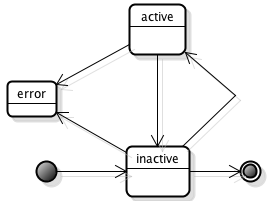
\includegraphics[scale=0.4]{figs/infra-link-state.png}
	\caption{State Diagram for a \hl{NetworkInterface} instance.}
	\label{fig:networklink_state}
\end{figure}

\paragraph{IPNetworkInterface Mixin}
In order to support L3/L4 capabilities (e.g. IP, TCP etc.) with the
\hl{NetworkInterface} type, an OCCI \hl{Mixin} instance is herewith
defined.

The \hl{IPNetworkInterface} mixin is assigned%
\footnote{Both assignments use data members from the inherited \hl{Category}
type \cite{occi:core}.}
the ``{\tt scheme}'' of
\textit{http://schemas.ogf.org/occi/infrastructure/networkinterface\#} and the ``{\tt term}'' value
\textit{ipnetworkinterface}.
An \hl{IPNetworkInterface} mixin MUST support these attributes.

The \hl{IPNetworkInterface} mixin MUST be related to the \hl{NetworkInterface} kind
by setting the \textit{applies} attribute to:

\textit{http://schemas.ogf.org/occi/infrastructure\#networkinterface}.

Table~\ref{tbl:ipnetworkinterface} define the attributes introduced by
the \hl{IPNetworkInterface} mixin.  A \hl{NetworkInterface} instance
associated with the \hl{IPNetworkInterface} mixin \hl{Mixin} instance
MUST expose these attributes.

\mytablefloat{
	\label{tbl:ipnetworkinterface}%
	\hl{Attribute}s defined by the \hl{IPNetworkInterface} mixin. A \hl{NetworkInterface}
	instance associated with this \hl{Mixin} instance MUST expose these
	attributes.
}{
\begin{tabular}{llp{1cm}lp{5cm}}
\toprule
Attribute&Type&Multi\-plicity&Mutability&Description\\
\colrule
occi.networkinterface.address & IPv4 or IPv6 Address & 1 & Mutable & Internet Protocol(IP) network address (e.g. 192.168.0.1/24, fc00::/7) of the link\\
occi.networkinterface.gateway & IPv4 or IPv6 Address & 0\ldots1 & Mutable & Internet Protocol(IP) network address (e.g. 192.168.0.1/24, fc00::/7)\\
occi.networkinterface.allocation & Enum \{dynamic, static\} & 1 & Mutable & Address mechanism: \textit{dynamic} e.g. uses the dynamic host configuration protocol, \textit{static} e.g. uses user supplied static network configurations.\\
\botrule
\end{tabular}
}

In Figure \ref{fig:networkinterface_mixin} a UML object diagram
depicts how \hl{NetworkInterface} would be associated with an
\hl{IPNetworkInterface} \hl{Mixin} when both are instantiated.

\begin{figure}[!h]
	\centering
	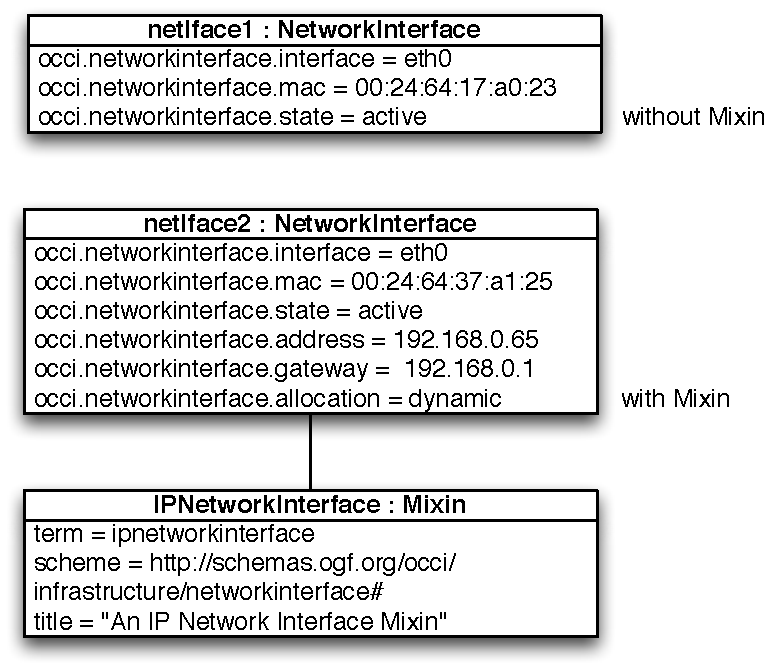
\includegraphics[scale=0.5]{figs/infrastructure_mixins_obj_dia2_networkinterface}
	\caption{Object Diagram of a \hl{NetworkInterface} Instance and its Associated
	IPNetworkInterface \hl{Mixin}.}
	\label{fig:networkinterface_mixin}
\end{figure}

\subsubsection{Linking to Storage}
The \hl{StorageLink} type represents a link from a \hl{Resource} to a
target \hl{Storage} instance. This enables a \hl{Storage} instance be
attached to a \hl{Compute} instance, with all the prerequisite low-
level operations handled by the OCCI implementation. \hl{Storage}
inherits the \hl{Link} base type defined in the OCCI Core Model
\cite{occi:core}.

The \hl{StorageLink} type is assigned the \hl{Kind} instance
\textit{http://schemas.ogf.org/occi/infrastructure\#storagelink}.  A
\hl{StorageLink} instance MUST use and expose this \hl{Kind}.  The
\hl{Kind} instance assigned to the \hl{StorageLink} type MUST be
related to the \textit{http://schemas.ogf.org/occi/core\#link}
\hl{Kind} by setting the \textit{parent} attribute.

\mytablefloat{
	\label{tbl:storagelink}\hl{Attribute}s defined for the \hl{StorageLink} type.
}
{
	\begin{tabular}{lp{2.5cm}p{1cm}lp{5cm}}
	\toprule
	Attribute&Type&Multi\-plicity&Mutability&Description\\
	\colrule
	occi.storagelink.deviceid & String & 1 & Mutable
	& Device identifier as defined by the OCCI service provider.\\
	occi.storagelink.mountpoint & String & 0\ldots1 & Mutable
	& Point to where the storage is mounted in the guest OS.\\
	occi.storagelink.state & Enum \{active, inactive, error\}& 1
	& Immutable & Current status of the instance.\\
	occi.storagelink.state.message & String & 0..1 & Immutable
	& Human-readable explanation of the current instance state.\\
	\botrule
	\end{tabular}
}

Table~\ref{tbl:storagelink} describes the OCCI Attributes%
\footnote{See the ``{\tt attributes}'' attribute defined by the
  \hl{Category} type and inherited by \hl{Kind} \cite{occi:core}.}
defined by \hl{StorageLink} through its \hl{Kind} instance. These
attributes MAY or MUST be exposed by an instance of the \hl{StorageLink} type
depending on the ``Multiplicity'' column in the aforementioned table.
Figure~\ref{fig:storagelink_state} illustrates the state
diagram for a \hl{StorageLink} instance.

\begin{figure}[!h]
	\centering
	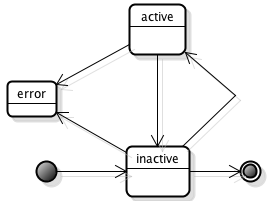
\includegraphics[scale=0.4]{figs/infra-link-state.png}
	\caption{State Diagram for a \hl{StorageLink} instance.}
	\label{fig:storagelink_state}
\end{figure}

\subsubsection{Linking to CDMI Managed Storage}
As previously stated, OCCI can be used in conjunction with the SNIA
cloud storage standard, Cloud Data Management Interface (CDMI)
\cite{cdmi} to provide enhanced management of the cloud computing
storage and data. In order to integrate the two, the use of
\hl{StorageLink} should be used. This will link OCCI managed Resources
to CDMI resources. The 'occi.storagelink.deviceid' attribute of
\hl{StorageLink}, defined above, should be set to the CDMI Object ID
of an exported CDMI Container.

\subsection{Infrastructure Templates}
Infrastructure Templates allow clients of an OCCI implementation to
quickly and conveniently apply pre-defined configurations to OCCI
Infrastructure defined types. They are implemented using \hl{Mixin}
instances. There are 2 supported infrastructure template types in OCCI
Infrastructure.

\subsubsection{OS Template}
OS (Operating System) Templates allow clients specific what operating
system must be installed on a requested \hl{Compute} resource. OCCI
implementations SHOULD support this, otherwise what they provision
will be merely offer \hl{Resource}s without any available execution
environment (e.g. operating system). Of the two supported template
types, this is the most basic and necessary template that a provider
SHOULD offer.

Its construction is a \hl{Mixin} instance consisting of a provider
specific ``scheme'' and a descriptive ``title'' detailing the OS. The
``term'' value of the template \hl{Mixin} is a provider-specific
identifier that corresponds to a particular image configuration. Where
an implementation requires additional attributes associated with the
OS Template, it can do so using ``{\tt attributes}'' value inherited
from the \hl{Category} type.

Default values for OCCI Attributes defined by the \hl{Kind} or the OS
Template \hl{Mixin} MAY be provided using the \hl{Attribute}.{\tt
  default} attribute property \cite{occi:core}.

A implementation-defined OS Template \hl{Mixin} MUST be related to the
OCCI OS Template \hl{Mixin} in order to give absolute type
information by setting the \textit{depends} attribute.

The OCCI OS Template is defined by the
\textit{http://schemas.ogf.org/occi/infrastructure\#os\_tpl}
\hl{Mixin} and MUST be supported SHOULD OS Templates be offered by the
OCCI implementation.

\begin{figure}[!h]
	\centering
	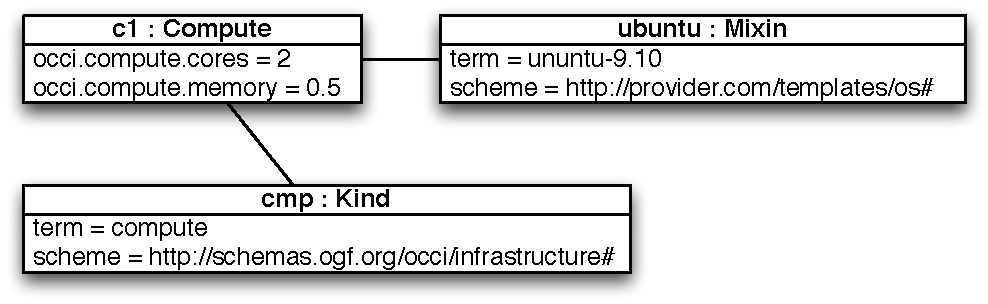
\includegraphics[scale=0.5]{figs/infra_template_obj_diag1}
	\caption{Object Diagram of a \hl{Compute} Instance and its Associated OS Template \hl{Mixin}.}
	\label{fig:infra_template_obj_diag1}
\end{figure}

%\begin{verbatim}
%POST /compute
%Category: compute; scheme='http://schemas.ogf.org/occi/infrastructure#';
%    title='Compute Instance',
%    ubuntu-9.10; scheme='http://provider.com/templates/os#';
%    title='Ubuntu 9.10'
%Attribute: occi.compute.memory=0.5, occi.compute.cores=2
%\end{verbatim}

A typical example of using such a \hl{Mixin} is shown in
figure~\ref{fig:infra_template_obj_diag1} using a UML object diagram.
In the example illustrated in
figure~\ref{fig:infra_template_obj_diag1} a provider has defined an OS
template which offers the ability to run Ubuntu Linux, verson 9.10,
upon a client's provisioned compute resource.

How a provider manages their set of OS templates will be determined by
themselves and so implementation-specific.

\subsubsection{Resource Template}
The Resource Template \hl{Mixin} builds upon the concept of OS
Templates. A Resource Template is a provider-defined \hl{Mixin}
instance that refers to a preset \hl{Resource} configuration.

The preset \hl{Resource} configuration is not visable through the OCCI
Discovery mechanism. The \hl{Mixin}.{\tt attributes} (inherited from
\hl{Category}) is empty for a Resource Template \hl{Mixin}.  The
side-effect of initialising \hl{Resource} attributes with pre-defined
values is handled by the implementation.

The OCCI implementation associates a set of Resource attributes (via
\hl{Category}'s 'attributes') with a particular term identifier.

An implementation-defined Resource Template \hl{Mixin} MUST be related
to the OCCI Resource Template \hl{Mixin} in order to give absolute
type information. This is done by setting the \textit{depends} attribute.
The OCCI Resource Template is defined by the
\hl{Mixin} instance
\textit{http://schemas.ogf.org/occi/infrastructure\#resource\_tpl} and
MUST be supported SHOULD Resource Templates be offered by the OCCI
implementation.

\begin{figure}[!h]
	\centering
	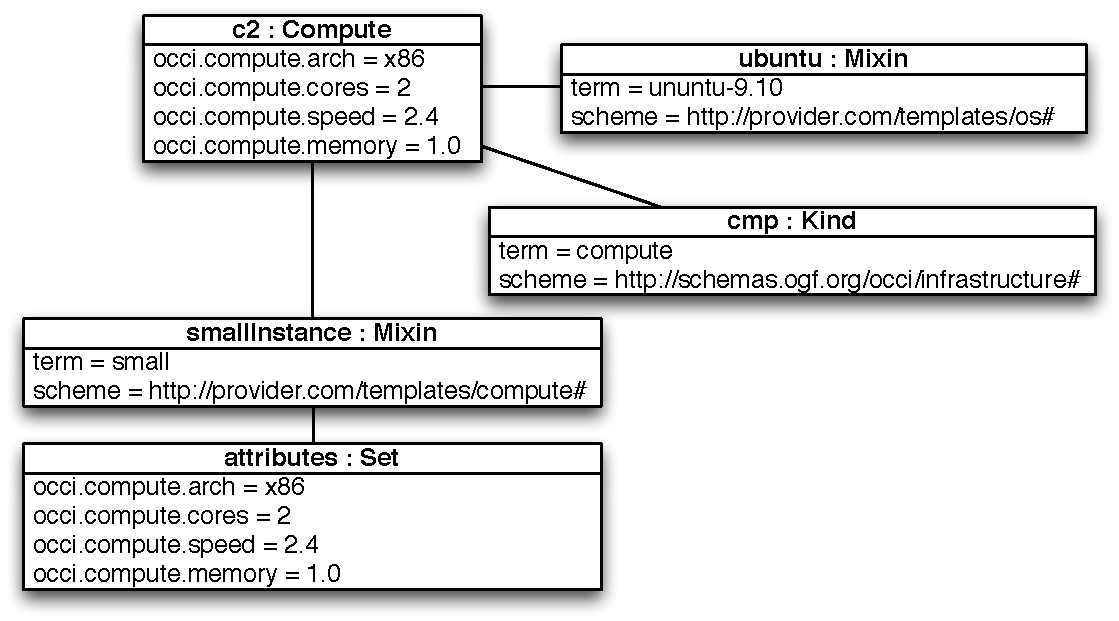
\includegraphics[scale=0.5]{figs/infra_template_obj_diag2}
	\caption{Object Diagram of a \hl{Compute} Instance and its Associated OS Template
	\hl{Mixin} and Resource Template \hl{Mixin}.}
	\label{fig:infra_template_obj_diag2}
\end{figure}

%\begin{verbatim}
%POST /compute
%Category: compute; scheme='http://schemas.ogf.org/occi/infrastructure#';
%    title='Compute Instance',
%    small; scheme="http://provider.com/templates/compute#";
%    title="Small Instance",
%    ubuntu-9.10; scheme="http://provider.com/templates/os#";
%    title="Ubuntu 9.10"
%\end{verbatim}

A typical example of such a \hl{Mixin}'s use is shown in
figure~\ref{fig:infra_template_obj_diag2}) using a UML object diagram.
In this example, the provider offers \hl{Compute} \hl{Resource}s based
on different sizes (i.e. small, medium, large). Each ``size'' of
\hl{Compute} (i.e. the term) corresponds to a predetermined set of
OCCI \hl{Resource}-specific attributes. In the example below a 'small'
\hl{Compute} instance is created.  Specifying "small" as the term
corresponds to an implementation-specific \hl{Compute}
\hl{Resource}-specific attribute set%
\footnote{This attribute set is implementation-specific and is {\em
    not} related to \hl{Mixin}.{\tt attributes} inherited from the
  \hl{Category} type \cite{occi:core}.}  that is shown by the object
instance named ``attributes'' in
figure~\ref{fig:infra_template_obj_diag2}.

%\begin{verbatim}
%Attribute: occi.compute.cores='2', occi.compute.share='200',
%    occi.compute.memory='1.0', occi.compute.arch='x86'
%\end{verbatim}

From the administrative point of view, how an OCCI service provider
manages their set of \hl{Resource} Templates will be determined by
themselves and so is implementation-specific.

\paragraph{Credentials Mixin}

% new as of OCCI 1.2

When creating a Compute Resource a client normally supplies security credentials in the form of a public SSH key. This SSH key is injected into the Compute Resource by the provider on the client's behalf. This feature is provided by the Credentials Mixin.

If a provider that offers VMs with access secured by SSH then that OCCI implementation SHOULD support this. Otherwise no user supplied public SSH key can be injected into the Compute Resource.

The OCCI credentials mixin has the term \textit{'ssh\_key'} and the schema \textit{'http://schemas.ogf.org/occi/credentials\#'}.

The credentials mixin MUST only apply to the Compute Kind and therefore
the mixin should have its  \textit{applies} attribute set to:

\textit{http://schemas.ogf.org/occi/infrastructure\#compute}.


\mytablefloat{
	\label{tbl:contextmixin}%
	\hl{Attribute}s defined by the \hl{Credentials} mixin. A \hl{Compute}
	instance associated with this \hl{Mixin} instance MUST expose these
	attributes.
}{
\begin{tabular}{llp{1cm}lp{5cm}}
\toprule
Attribute&Type&Multi\-plicity&Mutability&Description\\
\colrule
occi.credentials.ssh.publickey & String & 1 & Mutable & The contents of the public key file to be injected into the Compute Resource\\
\botrule
\end{tabular}
}

\paragraph{Contextualisation Mixin}

% new as of OCCI 1.2
In order to ease automation, OCCI supports the means to execute a
program once Resource has been instantiated. This feature is
provided by the contextualisation mixin. On receipt of the
contextualisation data the OCCI implementation MUST distinguish
the type of data being presented and then supply that content to the
Compute Resource being instantiated. That content is then executed
by the Compute Resource as the last step in the Compute's boot-order.

OCCI implementations SHOULD support this otherwise no
contextualisation of a resource instance can be done.
The OCCI contextualisation mixin has the term \textit{user\_data}
and the schema \textit{http://schemas.ogf.org/occi/compute\#}

Contextualisation mixin MUST only apply to the Compute Kind and therefore
the mixin should have its  \textit{applies} attribute set to:

\textit{http://schemas.ogf.org/occi/infrastructure\#compute}.

\mytablefloat{
	\label{tbl:contextmixin}%
	\hl{Attribute}s defined by the \hl{Contextualisation} mixin. A \hl{Compute}
	instance associated with this \hl{Mixin} instance MUST expose these
	attributes.
}{
\begin{tabular}{llp{1cm}lp{5cm}}
\toprule
Attribute&Type&Multi\-plicity&Mutability&Description\\
\colrule
occi.compute.userdata & String & 1 & Mutable &
Contextualisation data (e.g. script, executable) that the client supplies once
and only once. It cannot be updated.\\
\botrule
\end{tabular}
}

% end infrastructure content

\section{Security Considerations}
The OCCI Infrastructure specification is an extension to the OCCI Core
and Model specification \cite{occi:core}; thus the same security
considerations as for the OCCI Core and Model specification apply
here.

\section{Glossary}
\label{sec:glossary}
\begin{tabular}{l|p{12cm}}
Term & Description \\
\hline
\hl{Action} & An OCCI base type. Represent an invocable operation on a \hl{Entity} sub-type instance or collection thereof. \\

\hl{Category} & A type in the OCCI model. The parent type of \hl{Kind}. \\

\hl{Client} & An OCCI client.\\

\hl{Collection} & A set of \hl{Entity} sub-type instances all associated to a particular \hl{Kind} or \hl{Mixin} instance. \\

\hl{Entity} & An OCCI base type. The parent type of \hl{Resource} and \hl{Link}. \\

\hl{Kind} & A type in the OCCI model. A core component of the OCCI classification system. \\

\hl{Link} & An OCCI base type. A \hl{Link} instance associate one \hl{Resource} instance with another. \\

mixin & An instance of the \hl{Mixin} type associated with a {\bf resource
 instance}. The ``mixin'' concept as used by OCCI {\em only} applies to
 instances, never to \hl{Entity} types. \\

\hl{Mixin} & A type in the OCCI model. A core component of the OCCI classification system. \\

\hl{OCCI} & Open Cloud Computing Interface \\

OCCI base type & One of \hl{Entity}, \hl{Resource}, \hl{Link} or \hl{Action}. \\

OGF & Open Grid Forum \\

\hl{Resource} & An OCCI base type. The parent type for all domain-specific resource types. \\

resource instance & An instance of a sub-type of \hl{Entity}. The OCCI
 model defines two sub-types of \hl{Entity}, the \hl{Resource} type and the
 \hl{Link} type. However, the term {\em resource instance} is defined to
 include any instance of a {\em sub-type} of \hl{Resource} or \hl{Link} as
 well. \\

Tag & A \hl{Mixin} instance with no attributes or actions defined. \\

Template & A \hl{Mixin} instance which if associated at resource instantiation
time pre-populate certain attributes. \\

type & One of the types defined by the OCCI model.  The OCCI model types are
 \hl{Category}, \hl{Kind}, \hl{Mixin}, \hl{Action}, \hl{Entity}, \hl{Resource}
 and \hl{Link}. \\

URI & Uniform Resource Identifier \\
URL & Uniform Resource Locator \\
URN & Uniform Resource Name \\
\end{tabular}


\section{Contributors}

We would like to thank the following people who contributed to this
document:

\begin{tabular}{l|p{2in}|p{2in}}
Name & Affiliation & Contact \\
\hline
Michael Behrens & R2AD & behrens.cloud at r2ad.com \\
Mark Carlson & Toshiba & mark at carlson.net \\
Augusto Ciuffoletti & University of Pisa & augusto.ciuffoletti at gmail.com\\
Andy Edmonds & Zhaw & andy at zhaw.ch \\
Sam Johnston & Google & samj at samj.net \\
Gary Mazzaferro & Independent &  garymazzaferro at gmail.com \\
Thijs Metsch & Intel & thijs.metsch at intel.com \\
Ralf Nyrén & Independent & ralf at nyren.net \\
Alexander Papaspyrou & Adesso & alexander at papaspyrou.name \\
Boris Parak & CESNET & parak at cesnet.cz \\
Alexis Richardson & Weaveworks & alexis.richardson at gmail.com \\
Shlomo Swidler & Orchestratus & shlomo.swidler at orchestratus.com \\
Florian Feldhaus & NetApp & florian.feldhaus at gmail.com \\
\end{tabular}

Next to these individual contributions we value the contributions from
the OCCI working group.


\section{Intellectual Property Statement}
The OGF takes no position regarding the validity or scope of any
intellectual property or other rights that might be claimed to pertain
to the implementation or use of the technology described in this
document or the extent to which any license under such rights might or
might not be available; neither does it represent that it has made any
effort to identify any such rights. Copies of claims of rights made
available for publication and any assurances of licenses to be made
available, or the result of an attempt made to obtain a general
license or permission for the use of such proprietary rights by
implementers or users of this specification can be obtained from the
OGF Secretariat.

The OGF invites any interested party to bring to its attention any
copyrights, patents or patent applications, or other proprietary
rights which may cover technology that may be required to practice
this recommendation. Please address the information to the OGF
Executive Director.


\section{Disclaimer}
This document and the information contained herein is provided on an
``As Is'' basis and the OGF disclaims all warranties, express or
implied, including but not limited to any warranty that the use of the
information herein will not infringe any rights or any implied
warranties of merchantability or fitness for a particular purpose.


\section{Full Copyright Notice}
Copyright \copyright ~Open Grid Forum (2009-2014). All Rights Reserved.

This document and translations of it may be copied and furnished to
others, and derivative works that comment on or otherwise explain it
or assist in its implementation may be prepared, copied, published and
distributed, in whole or in part, without restriction of any kind,
provided that the above copyright notice and this paragraph are
included on all such copies and derivative works. However, this
document itself may not be modified in any way, such as by removing
the copyright notice or references to the OGF or other organizations,
except as needed for the purpose of developing Grid Recommendations in
which case the procedures for copyrights defined in the OGF Document
process must be followed, or as required to translate it into
languages other than English.

The limited permissions granted above are perpetual and will not be
revoked by the OGF or its successors or assignees.


\bibliographystyle{IEEEtran}
\bibliography{references}

\appendix

\newpage
\section{Errata}
\label{sec:errata}

\end{document}
